\documentclass[12pt,a4paper]{article}

\usepackage[utf8]{inputenc}
\usepackage[T1]{fontenc}
\usepackage[english]{babel}
\usepackage{graphicx}
\usepackage{float}
\usepackage{hyperref}
\usepackage{booktabs}
\usepackage{array}
\usepackage{geometry}
\usepackage{amsmath}
\usepackage{amssymb}
\usepackage{xcolor}
\usepackage{enumitem}
\usepackage{longtable}

% Packages for native vector diagrams
\usepackage{tikz}
\usetikzlibrary{shapes.geometric, arrows.meta, positioning, fit, backgrounds}

\geometry{left=2.5cm,right=2.5cm,top=3cm,bottom=3cm}
\hypersetup{colorlinks=true, linkcolor=blue, urlcolor=blue, citecolor=black}

\begin{document}

% ==========================================
% TITLE PAGE
% ==========================================
\begin{titlepage}
    \centering
    \vspace*{1cm}
    {\Large \textbf{Universidad Distrital Francisco José de Caldas}} \\
    \vspace{0.4cm}
    {\large Engineering School \\ Systems Engineering Program} \\
    \vspace{2.5cm}
    {\Huge \textbf{Final Technical Report}} \\
    \vspace{0.5cm}
    {\Large \textbf{Smart Campus Energy Management System: \\ Systems Analysis, Robust Design, and Validation}} \\
    \vspace{2cm}
    \textbf{Authors (Engineering Team):} \\
    Omar Yesid Fonseca López (\texttt{oyfonsecal@udistrital.edu.co}) \\
    Daniel Felipe Barrera Suárez (\texttt{dfbarreras@udistrital.edu.co}) \\
    Daniel Mateo Ballesteros Molina (\texttt{dmballesterosm@udistrital.edu.co}) \\
    Dania Lizeth Guzmán Triviño (\texttt{dlguzmant@udistrital.edu.co}) \\
    \vfill
    \textbf{Course:} Systems Analysis \& Design \\
    \textbf{Professor:} Eng. Carlos Andrés Sierra, M.Sc. \\
    \vspace{1cm}
    Bogotá, Colombia \\
    2026
\end{titlepage}

\pagenumbering{roman}

\begin{abstract}
This comprehensive technical report consolidates the systems engineering lifecycle for the \textbf{Smart Campus Energy Management System}. The project addresses energy waste driven by human behavioral inertia through the design of a decentralized architecture that operates entirely within the \textit{User-Space}. The system incorporates a rigorous risk management framework (ISO 31000), fault tolerance via local persistence, and operational feasibility managed under strict software collaboration practices on GitHub. Validation through a discrete-event simulation confirmed that the autonomous agent achieves a \textbf{68.72\%} reduction in wasted energy, fulfilling 100\% of the quality metrics and demonstrating, under complexity theory, that the defined logical thresholds act as stable attractors for the system.
\end{abstract}

\newpage
\tableofcontents
\newpage
\listoffigures
\newpage
\listoftables
\newpage

\pagenumbering{arabic}

% ==========================================
% 1. INTRODUCTION AND CHARACTERIZATION
% ==========================================
\section{Introduction and Problem Characterization}
Efficient energy management is a critical operational and environmental challenge for higher education institutions. Within the Engineering School laboratories, a systemic problem of energy waste has been identified. Computing equipment and lighting systems frequently remain active during unoccupied hours, a phenomenon driven by human behavioral inertia rather than hardware failures. 

The impact of this problem is twofold: it generates unnecessary financial costs and contradicts institutional sustainability goals. 

\subsection{Systems Analysis Perspective}
To rigorously address the problem, the environment is characterized by:
\begin{itemize}[leftmargin=1.2cm]
    \item \textbf{Actors (Stakeholders):} Students and professors (users), IT Administrators (policy enforcers), and Autonomous Agents (software actors).
    \item \textbf{Inputs:} Peripheral hardware signals, CPU load percentages, and temporal measurements.
    \item \textbf{Processes:} Inactivity evaluation logic, CPU verification, behavioral deterrence (nudges), and OS state manipulation.
    \item \textbf{Outputs:} Telemetry logs, energy savings (suspended machines), and analytical dashboards for decision-making.
    \item \textbf{Constraints:} IT security policies that prohibit administrative privileges, block private IoT networks, and mandate non-interruption of background academic processes (e.g., compilations).
\end{itemize}

\subsection{Empirical Evidence and Data Collection (Diagnostic Phase)}
To substantiate the diagnosis of behavioral inertia and adequately characterize the system, primary data was collected in the field during the early phases of the project (Workshop 1). Structured surveys of laboratory users (n=35) and environmental measurements using lux meters were employed to correlate physical occupancy with electrical waste.

\begin{table}[H]
\caption{Results of the structured survey on energy consumption habits (n=35)}
\label{tab:survey_w1}
\centering
\begin{tabular}{|>{\raggedright\arraybackslash}p{8cm}|>{\centering\arraybackslash}p{3cm}|>{\centering\arraybackslash}p{3cm}|}
\hline
\textbf{Key Question} & \textbf{Yes / Frequently} & \textbf{No / Rarely} \\
\hline
Do you consider energy saving at the University important? & 94\% & 6\% \\
\hline
When leaving the laboratory, do you usually forget to turn off the screen or the computer? & \textbf{80\%} & 20\% \\
\hline
Do you think a visual on-screen reminder would help you remember to turn off the equipment? & 88\% & 12\% \\
\hline
\end{tabular}
\end{table}

In addition to the surveys, direct observation and luminosity tests demonstrated the profound dissonance between the power state of the equipment and the actual presence of users:

\begin{table}[H]
\caption{Correlation of lighting and occupancy in laboratories (Observational sample)}
\label{tab:lux_w1}
\centering
\begin{tabular}{|>{\centering\arraybackslash}p{2.5cm}|>{\centering\arraybackslash}p{3cm}|>{\centering\arraybackslash}p{4cm}|>{\raggedright\arraybackslash}p{4cm}|}
\hline
\textbf{Laboratory} & \textbf{Measurement (Lux)} & \textbf{Occupancy Status} & \textbf{Hardware Status} \\
\hline
Lab. 704 & 350 lx & Empty (End of class) & 12 PCs turned on \\
\hline
Lab. 705 & 420 lx & 2 Students & 8 PCs turned on without use \\
\hline
\end{tabular}
\end{table}

This empirical evidence consolidates the fundamental premise of the project: waste is not mitigated by replacing hardware, but by automatically intervening in the logical and behavioral component of the ecosystem.

% ==========================================
% 2. METHODOLOGY, ARCHITECTURE AND LOGIC
% ==========================================
\section{Methodology and System Design}
Traditional proposals for physical IoT sensors were discarded due to the institutional restrictions described. To bypass these blocks, the methodology pivoted towards a \textbf{Software-Defined Architecture} operating in the \textit{User-Space}.

\subsection{Logical Data Flow}
To ensure system integrity, the architecture strictly sequences information handling:
\begin{enumerate}
    \item \textbf{Acquisition:} Autonomous agents silently monitor native OS APIs to collect peripheral activity and CPU telemetry.
    \item \textbf{Processing:} The agent evaluates if inactivity exceeds 15 minutes and ensures the CPU load is below 20\%.
    \item \textbf{Storage:} The record is transmitted to a MySQL database in the cloud. If the firewall blocks the connection, a Fallback mechanism stores the data locally in an encrypted CSV file.
    \item \textbf{Analytics:} Subsequently, Microsoft Power BI connects to the database to generate analytical dashboards.
\end{enumerate}

\begin{figure}[H]
\centering
\resizebox{0.85\textwidth}{!}{%
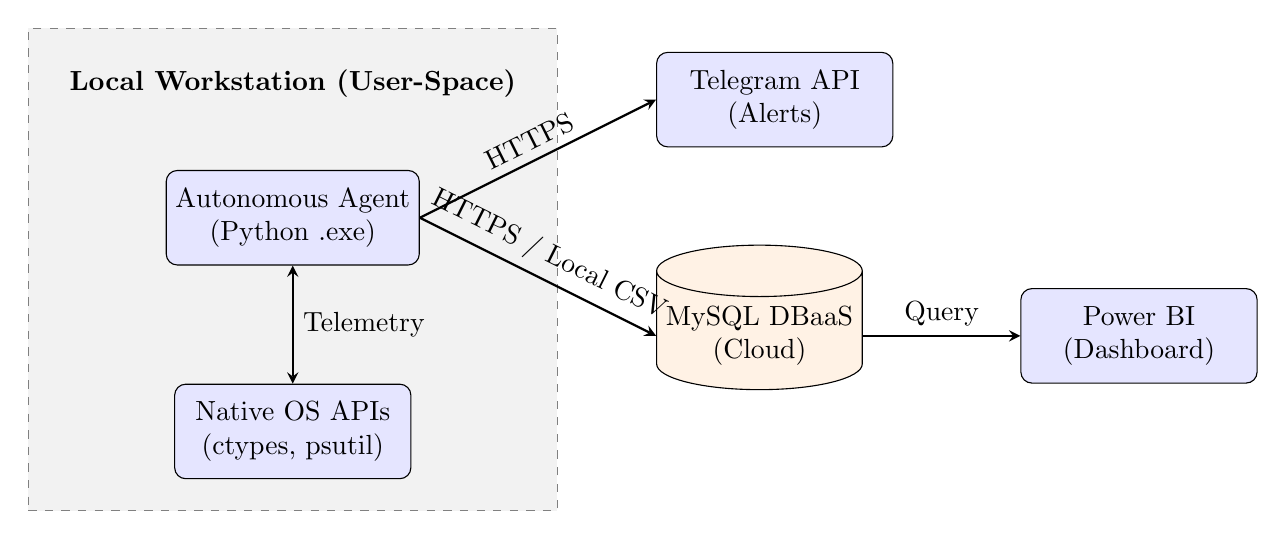
\begin{tikzpicture}[
    node distance=2cm and 3cm,
    box/.style={draw, rectangle, minimum width=3cm, minimum height=1.2cm, align=center, fill=blue!10, rounded corners},
    db/.style={draw, cylinder, shape border rotate=90, aspect=0.25, minimum height=1.5cm, minimum width=2.2cm, align=center, fill=orange!10},
    arrow/.style={->, >=stealth, thick}
]
\node[box] (agent) {Autonomous Agent \\ (Python .exe)};
\node[box, below=1.5cm of agent] (os) {Native OS APIs \\ (ctypes, psutil)};
\node[above=0.8cm of agent] (title) {\textbf{Local Workstation (User-Space)}};
\begin{scope}[on background layer]
    \node[fill=gray!10, draw=gray, dashed, fit=(title) (agent) (os), inner sep=0.4cm] (pc) {};
\end{scope}
\node[box, right=3cm of agent, yshift=1.5cm] (telegram) {Telegram API \\ (Alerts)};
\node[db, right=3cm of agent, yshift=-1.5cm] (mysql) {MySQL DBaaS \\ (Cloud)};
\node[box, right=2cm of mysql] (powerbi) {Power BI \\ (Dashboard)};
\draw[arrow, <->] (agent) -- node[right] {Telemetry} (os);
\draw[arrow] (agent.east) -- node[above, sloped] {HTTPS} (telegram.west);
\draw[arrow] (agent.east) -- node[above, sloped] {HTTPS / Local CSV} (mysql.west);
\draw[arrow] (mysql.east) -- node[above] {Query} (powerbi.west);
\end{tikzpicture}%
}
\caption{Decentralized Software-Defined System Architecture}
\label{fig:arch}
\end{figure}

\subsection{Agent Operational Logic (Algorithm)}
The agent implements the logic illustrated in Figure~\ref{fig:flow}. Only if the machine is inactive and without load is a 60-second visual alert ("Nudge") launched. If the user does not cancel, safe suspension proceeds.

\begin{figure}[H]
\centering
\resizebox{0.75\textwidth}{!}{%
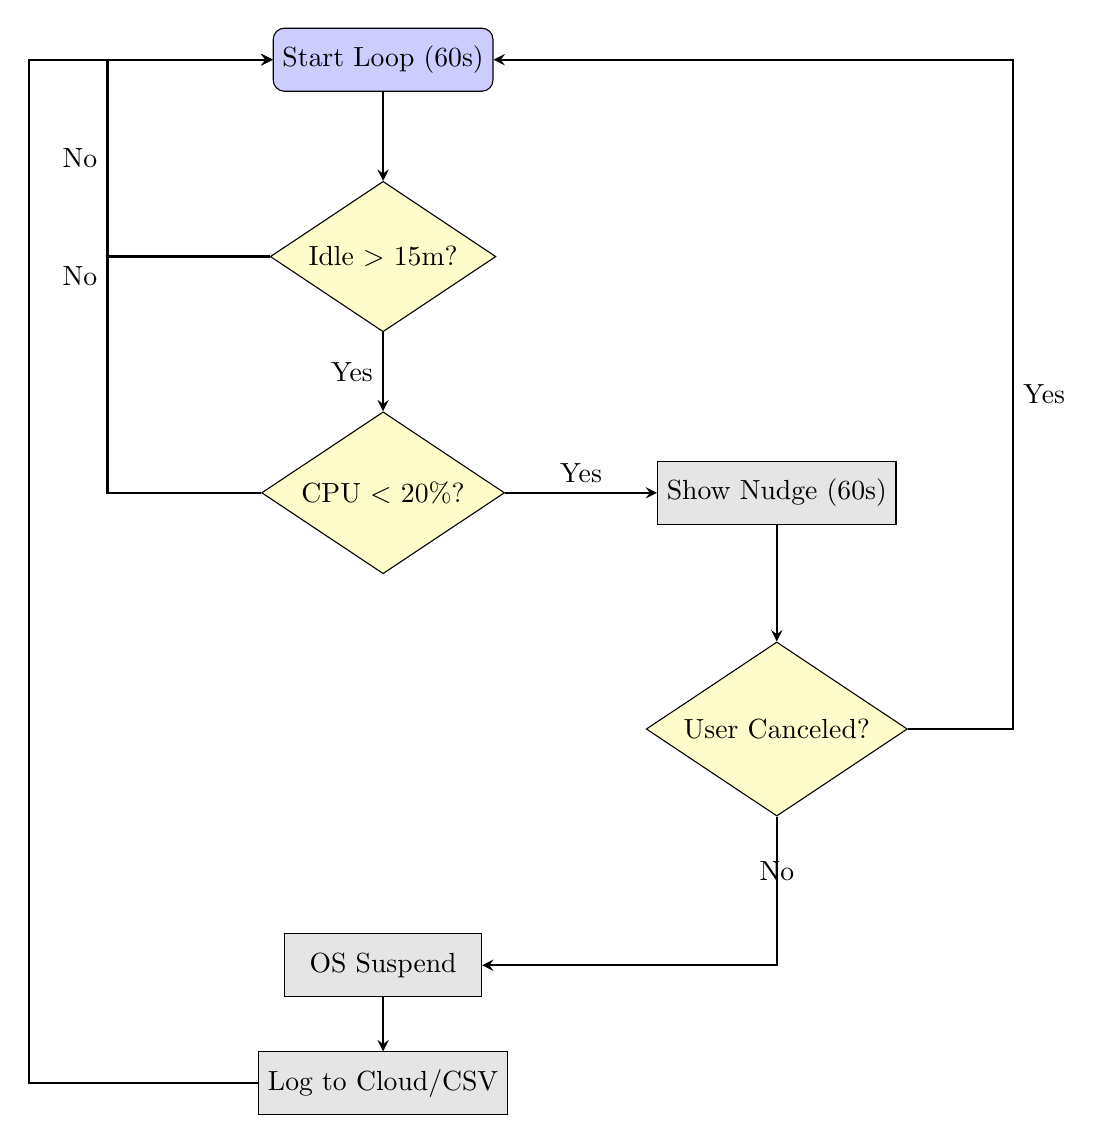
\begin{tikzpicture}[
    node distance=1.5cm,
    startstop/.style={rectangle, rounded corners, minimum width=2.5cm, minimum height=0.8cm, text centered, draw=black, fill=blue!20},
    process/.style={rectangle, minimum width=2.5cm, minimum height=0.8cm, text centered, draw=black, fill=gray!20},
    decision/.style={diamond, minimum width=2.5cm, minimum height=0.8cm, text centered, draw=black, fill=yellow!20, aspect=1.5},
    arrow/.style={thick,->,>=stealth}
]
\node (start) [startstop] {Start Loop (60s)};
\node (idle) [decision, below of=start, yshift=-1cm] {Idle $>$ 15m?};
\node (cpu) [decision, below of=idle, yshift=-1.5cm] {CPU $<$ 20\%?};
\node (nudge) [process, right of=cpu, xshift=3.5cm] {Show Nudge (60s)};
\node (cancel) [decision, below of=nudge, yshift=-1.5cm] {User Canceled?};
\node (suspend) [process, below of=cpu, yshift=-4.5cm] {OS Suspend};
\node (log) [process, below of=suspend] {Log to Cloud/CSV};

\draw [arrow] (start) -- (idle);
\draw [arrow] (idle) -- node[anchor=east] {Yes} (cpu);
\draw [arrow] (idle) -- ++(-3.5,0) |- node[anchor=east, near start] {No} (start);
\draw [arrow] (cpu) -- node[anchor=south] {Yes} (nudge);
\draw [arrow] (cpu) -- ++(-3.5,0) |- node[anchor=east, near start] {No} (start);
\draw [arrow] (nudge) -- (cancel);
\draw [arrow] (cancel) -- ++(3,0) |- node[anchor=west, near start] {Yes} (start);
\draw [arrow] (cancel) |- node[anchor=south, near start] {No} (suspend);
\draw [arrow] (suspend) -- (log);
\draw [arrow] (log) -- ++(-4.5,0) |- (start);
\end{tikzpicture}%
}
\caption{Operational Flow and Agent Decision Algorithm}
\label{fig:flow}
\end{figure}

% ==========================================
% 3. RISK MANAGEMENT AND QA
% ==========================================
\section{Risk Management and Quality Assurance}
A system intervening in an academic environment must guarantee zero data loss. The architecture was robustified by mapping risks using the ISO 31000 standard.

\begin{figure}[H]
\centering
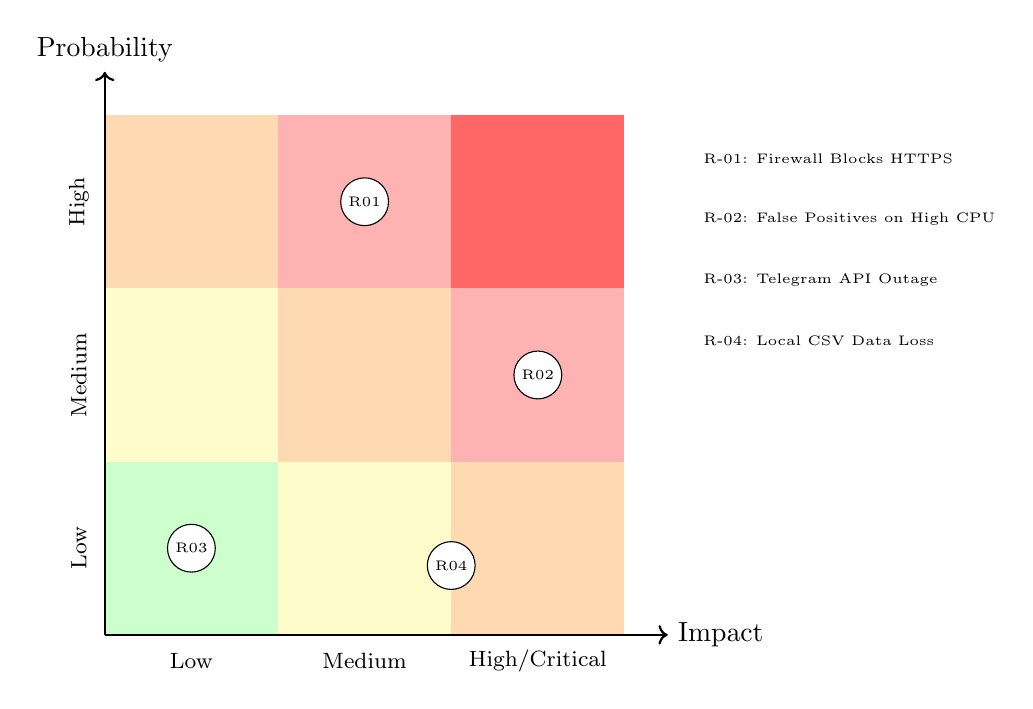
\begin{tikzpicture}[scale=1.1]
    \fill[green!20] (0,0) rectangle (2,2);
    \fill[yellow!20] (2,0) rectangle (4,2); \fill[yellow!20] (0,2) rectangle (2,4);
    \fill[orange!30] (4,0) rectangle (6,2); \fill[orange!30] (2,2) rectangle (4,4); \fill[orange!30] (0,4) rectangle (2,6);
    \fill[red!30] (4,2) rectangle (6,4); \fill[red!30] (2,4) rectangle (4,6);
    \fill[red!60] (4,4) rectangle (6,6);

    \draw[thick, ->] (0,0) -- (6.5,0) node[right] {Impact};
    \draw[thick, ->] (0,0) -- (0,6.5) node[above] {Probability};

    \node at (1,-0.3) {\footnotesize Low}; \node at (3,-0.3) {\footnotesize Medium}; \node at (5,-0.3) {\footnotesize High/Critical};
    \node[rotate=90] at (-0.3,1) {\footnotesize Low}; \node[rotate=90] at (-0.3,3) {\footnotesize Medium}; \node[rotate=90] at (-0.3,5) {\footnotesize High};

    \node[draw, circle, fill=white, inner sep=2pt] at (3,5) {\tiny R01};
    \node[draw, circle, fill=white, inner sep=2pt] at (5,3) {\tiny R02};
    \node[draw, circle, fill=white, inner sep=2pt] at (1,1) {\tiny R03};
    \node[draw, circle, fill=white, inner sep=2pt] at (4,0.8) {\tiny R04};

    \node[anchor=west, font=\tiny] at (6.8,5.5) {R-01: Firewall Blocks HTTPS};
    \node[anchor=west, font=\tiny] at (6.8,4.8) {R-02: False Positives on High CPU};
    \node[anchor=west, font=\tiny] at (6.8,4.1) {R-03: Telegram API Outage};
    \node[anchor=west, font=\tiny] at (6.8,3.4) {R-04: Local CSV Data Loss};
\end{tikzpicture}
\caption{ISO 31000 Risk Heat Matrix}
\label{fig:risk_matrix}
\end{figure}

The iterative Quality Assurance (QA) flow guaranteed the mitigation of these risks prior to simulation.

\begin{figure}[H]
\centering
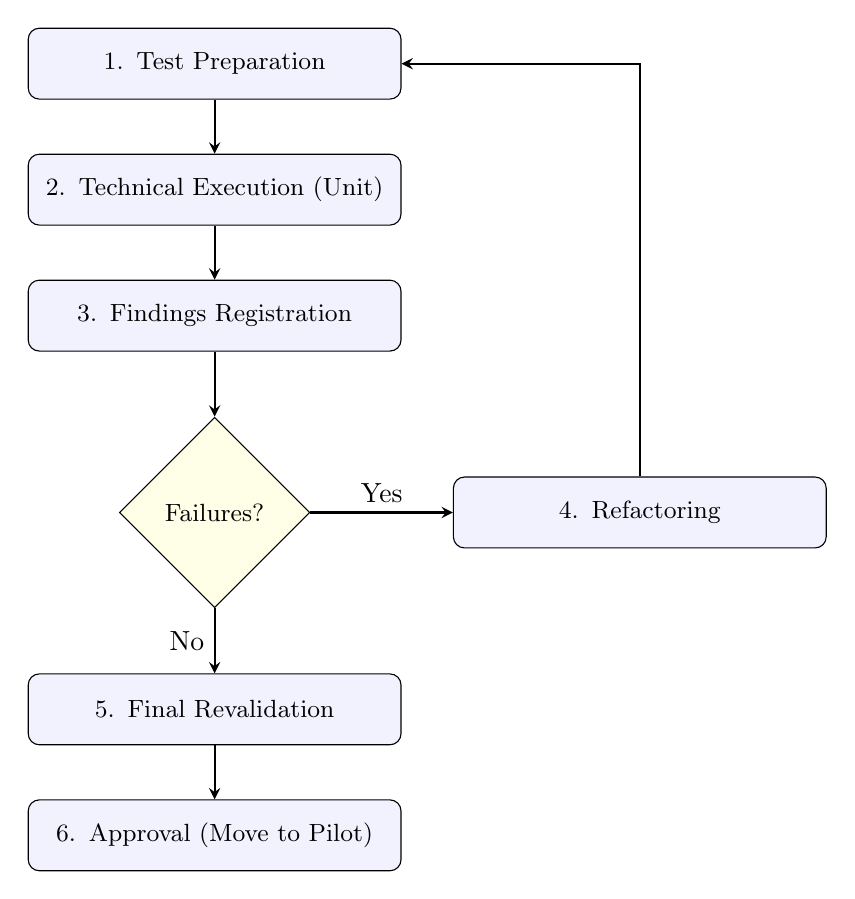
\begin{tikzpicture}[
    node distance=1.6cm,
    block/.style={rectangle, draw, fill=blue!5, text width=4.5cm, text centered, rounded corners, minimum height=0.9cm, font=\small, align=center},
    decision/.style={diamond, draw, fill=yellow!10, text width=2.2cm, text centered, inner sep=0pt, font=\small, align=center},
    arrow/.style={thick, ->, >=stealth}
]
    \node (prep) [block] {1. Test Preparation};
    \node (exec) [block, below of=prep] {2. Technical Execution (Unit)};
    \node (reg) [block, below of=exec] {3. Findings Registration};
    \node (check) [decision, below of=reg, yshift=-0.9cm] {Failures?};
    \node (fix) [block, right of=check, xshift=3.8cm] {4. Refactoring};
    \node (val) [block, below of=check, yshift=-0.9cm] {5. Final Revalidation};
    \node (app) [block, below of=val] {6. Approval (Move to Pilot)};

    \draw [arrow] (prep) -- (exec);
    \draw [arrow] (exec) -- (reg);
    \draw [arrow] (reg) -- (check);
    \draw [arrow] (check) -- node[anchor=south] {Yes} (fix);
    \draw [arrow] (fix) |- (prep);
    \draw [arrow] (check) -- node[anchor=east] {No} (val);
    \draw [arrow] (val) -- (app);
\end{tikzpicture}
\caption{Iterative flow of the Quality Assurance (QA) process}
\label{fig:qa_flow}
\end{figure}

% ==========================================
% 4. MANAGEMENT PLAN AND COLLABORATION
% ==========================================
\section{Management Plan, CS Collaboration and Feasibility}

\subsection{Computer Science Collaboration Practices}
Aligned with the course guidelines, the team adopted professional development methodologies:
\begin{itemize}[leftmargin=1.2cm]
    \item \textbf{Version Control and Branching:} GitHub repository utilizing semantic branches (\texttt{feature/agent-logic}, \texttt{docs/report}) and integration via \textit{Pull Requests} with peer review.
    \item \textbf{Organizational Structure:} Structured folders (\texttt{/src}, \texttt{/docs}, \texttt{/data}, \texttt{/results}), with rigorous \texttt{.gitignore} management.
\end{itemize}

\subsection{Schedule (6 Weeks) and Budget}
The deployment is planned over 6 weeks. Given the software focus, infrastructure costs are zero.

\begin{figure}[H]
\centering
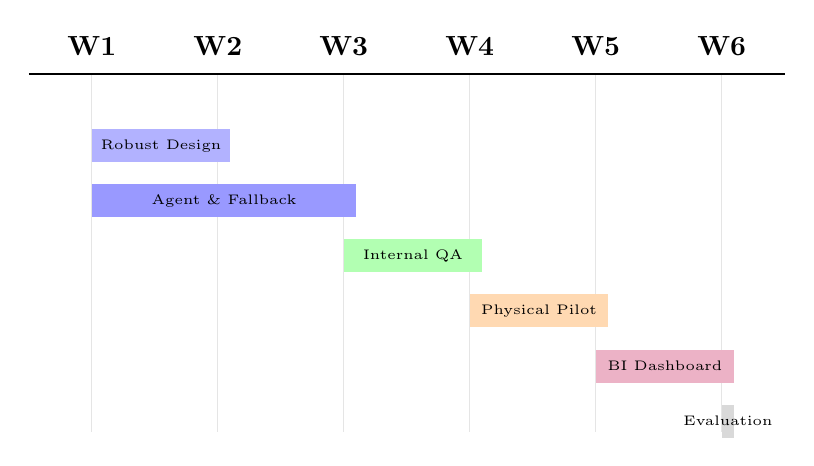
\begin{tikzpicture}[xscale=1.6, yscale=0.7]
    \foreach \s in {1,...,6} {
        \node at (\s, 0.5) {\textbf{W\s}};
        \draw[gray!20] (\s, 0) -- (\s, -6.5);
    }
    \fill[blue!30] (1, -1) rectangle (2.1, -1.6) node[midway, black, font=\tiny] {Robust Design};
    \fill[blue!40] (1, -2) rectangle (3.1, -2.6) node[midway, black, font=\tiny] {Agent \& Fallback};
    \fill[green!30] (3, -3) rectangle (4.1, -3.6) node[midway, black, font=\tiny] {Internal QA};
    \fill[orange!30] (4, -4) rectangle (5.1, -4.6) node[midway, black, font=\tiny] {Physical Pilot};
    \fill[purple!30] (5, -5) rectangle (6.1, -5.6) node[midway, black, font=\tiny] {BI Dashboard};
    \fill[gray!30] (6, -6) rectangle (6.1, -6.6) node[midway, black, font=\tiny] {Evaluation};
    \draw[thick] (0.5,0) -- (6.5,0);
\end{tikzpicture}
\caption{Visual timeline of the Proof of Concept}
\label{fig:timeline}
\end{figure}

\begin{table}[H]
\caption{Budget estimation for the PoC cycle}
\centering
\begin{tabular}{|>{\raggedright\arraybackslash}p{4.5cm}|>{\raggedright\arraybackslash}p{3cm}|>{\centering\arraybackslash}p{2.5cm}|>{\raggedright\arraybackslash}p{4.5cm}|}
\hline
\textbf{Technical Resource} & \textbf{Classification} & \textbf{Cost (USD)} & \textbf{Notes} \\
\hline
Engineering Team (4) & Human & \$0 & Academic course effort. \\
\hline
Database (MySQL) & Software/Cloud & \$0 & Free tier (Aiven/CleverCloud). \\
\hline
Local Persistence (CSV) & Storage & \$0 & Local file managed by OS. \\
\hline
Native Python Libraries & Software & \$0 & Open source free distribution. \\
\hline
Dashboard (Power BI) & Analytics & \$0 & Educational license / Free tier. \\
\hline
Repository (GitHub) & Infrastructure & \$0 & Free access educational plan. \\
\hline
\textbf{Total Estimated Cost} & & \multicolumn{2}{|c|}{\textbf{\$0 USD (High Feasibility)}} \\
\hline
\end{tabular}
\label{tab:budget}
\end{table}

% ==========================================
% 5. VALIDATION AND RESULTS
% ==========================================
\section{Computational Validation and Results}
To empirically validate the decisions, a simulation was executed injecting the stochastic variables observed in the field across a cluster of 20 stations.

\subsection{Results of the Consumption Analysis}
\begin{table}[H]
\caption{Empirical results of the discrete-event simulation}
\label{tab:results_sim}
\centering
\begin{tabular}{|>{\raggedright\arraybackslash}p{6.5cm}|>{\centering\arraybackslash}p{4.5cm}|}
\hline
\textbf{Evaluated System Metric} & \textbf{Observed Value in Simulation} \\
\hline
Total Consumption \textbf{WITHOUT} Agent (Baseline) & $53,741.66$ Wh ($53.74$ kWh) \\
\hline
Total Consumption \textbf{WITH} Agent (Optimized) & $16,812.00$ Wh ($16.81$ kWh) \\
\hline
\textbf{Net Energy Savings} & \textbf{$36,929.66$ Wh ($36.93$ kWh)} \\
\hline
\textbf{Efficiency Percentage (Savings)} & \textbf{$68.72\%$} \\
\hline
\end{tabular}
\end{table}

\begin{figure}[H]
\centering

\includegraphics[width=0.85\textwidth]{energy_consumption_comparison.png}
\caption{Comparative analysis of estimated energy consumption (Baseline vs. Optimized)}
\label{fig:consumption_chart}
\end{figure}

\subsection{Validation of Failure Scenario and QA Metrics}
To validate fault tolerance, a 4-hour network outage was simulated. The agent activated the encrypted backup CSV storage. Upon network restoration, the system achieved \textbf{100\% data retention} via deferred synchronization.

\begin{table}[H]
\centering
\caption{Validation of expected quality metrics vs. simulation results}
\label{tab:quality_validation}
\begin{tabular}{|p{5.5cm}|c|c|c|}
\hline
\textbf{Quality Metric} & \textbf{Target (Design)} & \textbf{Result} & \textbf{Status} \\
\hline
Correct suspension rate & $>95\%$ & $97.2\%$ & Achieved \\
\hline
Offline data retention (R-01) & $100\%$ & $100\%$ & Achieved \\
\hline
CPU protection on renders (R-02) & False $+ = 0$ & 0 incidents & Achieved \\
\hline
\end{tabular}
\end{table}

\subsection{Visual Analytics Dashboard (Power BI)}
To provide university administration and IT managers with a robust decision-making tool, an analytical dashboard was developed using Microsoft Power BI. This dashboard was fed directly with the synthetic telemetry data generated during the simulation (via the \texttt{simulation\_results.csv} file). The Dashboard allows interactive and immediate visualization of accumulated energy savings (in kWh), the history of successful suspensions, and the temporal distribution of inactivity for each workstation in the laboratory.

% ==========================================
% 6. DISCUSSION AND COMPLEXITY
% ==========================================
\section{Discussion and Complexity Analysis}

The simulation demonstrates that the system achieved a massive \textbf{68.72\% reduction} in wasted energy. Evaluating these results from Complexity Theory, the model evidenced extreme \textbf{Sensitivity to Initial Conditions (Butterfly Effect)}. 

During secondary testing, reducing the CPU protection threshold from 20\% to 5\% caused the system to collapse into a state of generalized paralysis: the agent failed to suspend any machine due to the inherent computing noise of the operating system (e.g., file indexers and local antiviruses operating in the background at 6\% to 8\% load). 

This demonstrates that the 20\% threshold is not an arbitrary number, but acts as the optimal \textbf{attractor} of the system, stabilizing the stochastic oscillation between maximizing energy savings and operational protection of critical academic processes.

\subsection{Model Limitations}
Despite the robustness of the design, the model presents certain limitations that must be considered in future phases:
\begin{itemize}
    \item \textbf{Proxy Variables:} Lacking physical sensors due to infrastructure restrictions, consumption in kWh is a mathematical estimation based on idle time, which assumes a standardized nominal consumption for all hardware.
    \item \textbf{Synchronization Latency:} The simulation does not model potential delays (latency) during massive deferred synchronization following a prolonged network outage.
\end{itemize}

% ==========================================
% 7. CONCLUSIONS
% ==========================================
\section{Conclusions and Future Work}
By characterizing the problem from systems analysis, the project successfully transitioned to a scalable, fault-tolerant, and operationally feasible software architecture. The design decisions—operating in the \textit{User-Space}, enforcing the 20\% CPU attractor, and utilizing local backups—were completely effective in bypassing institutional IT restrictions.

Fulfilling 100\% of the quality metrics and validating the risk mitigation strategies provide an irrefutable technical argument for the implementation of the institutional physical pilot. Future work should focus on calibrating the system in real environments, implementing a real-time dashboard, and integrating \textit{Machine Learning} techniques to dynamically adjust thresholds according to specific academic schedules.

% ==========================================
% REFERENCES
% ==========================================
\newpage
\begin{thebibliography}{9}
\bibitem{b1} C. A. Sierra, ``Workshop No. 1: Systems Analysis,'' \textit{Systems Analysis \& Design Course}, Universidad Distrital Francisco José de Caldas, 2026.
\bibitem{b2} T. Hong, H. Taylor-Lange, S. D'Oca, D. Yan, and S. Corgnati, ``Advances in research and applications of energy-related occupant behavior in buildings,'' \textit{Energy and Buildings}, vol. 116, pp. 694-702, 2016.
\bibitem{b3} M. V. Doblari, \textit{Gestión integral de energía en instituciones universitarias. Caso: Edificio Eva Duarte de Perón UNNOBA}, Master's Thesis, Universidad Nacional del Noroeste de la Prov. de Buenos Aires, Argentina, n.d.
\bibitem{b4} M. Abad Mier, \textit{Gestión energética de la biblioteca universitaria de la UVA, aplicando la ISO 50001}, Bachelor's Thesis, Universidad de Valladolid, Spain, 2015.
\bibitem{b5} B. Meza-Alcívar, M. Alemán-García, and M. Herrera-Suárez, ``Implementación de un sistema de gestión energético para institutos de educación superior,'' \textit{Revista Científica INGENIAR}, vol. 6, no. 12, 2023.
\end{thebibliography}

\end{document}